\documentclass[./main.tex]{subfiles} 
\begin{document}

\subsection{Time-Frequency Estimation}

\subsubsection{Experimenting with the Spectrogram}

We are introduced to the concept of the spectrogram, which allows us to view the frequency spectrum across the time domain. For example, a the frequency spectra of a voice signal will change significantly over time, and the spectrogram allows us to view this change without looking at a different PSD for each period in time.

There are various parameters which go in to the spectrogram. The \texttt{chirp} function from \texttt{MATLAB} was used to generate the signal used across these tests. Figure \ref{fig:2_3_a_window_size} shows differing window sizes - the window taken for each Short Time Fourier Transform. The window also allows a smooth FFT (so as to avoid the problems of using a rect gate)- we will look at some different Windows (for example, Bartlett). There is also a proportion of overlap between each segment, so that the spectrogram appears smoother between each step. The legnth of the FFT also has an impact, as it will determine the resolution of the spectrogram at each step.

Figure \ref{fig:2_3_a_window_size} shows different window sizes. To ensure a fair test, we keep the FFT of the same length. The two middle window lengths, 128 and 256 appear the smoothest. A shorter window length results in noticably large chunks in the time domain. Conversely, a long window suffers from having too large a bandwith and thus having poor resolution in the freqency domain (noice how wide the chirp appears to be in comparison to the others).

Figure \ref{fig:2_3_a_fft_len} shows differing FFT lengths. Clearly, the larger the FFT the better the resolution. There is a trade off to be made between computational complexity and FFT length, however.

Figure \ref{fig:2_3_a_overlap} has 4 different percentages of overlap. This is allows a smooth transition between time steps, We can see that the overlap of 80\% appears the smoothest out of all overlaps. Of course, with such a large overlap, this means that more windows and STFTs will need to be computed.

Lastly, we look at differnet window functions in figure \ref{fig:2_3_a_windows}. Judging by the spectrogram, the Hanning window appears to have performed the best given the current set up. 

\begin{figure}[h]
	\centering 
	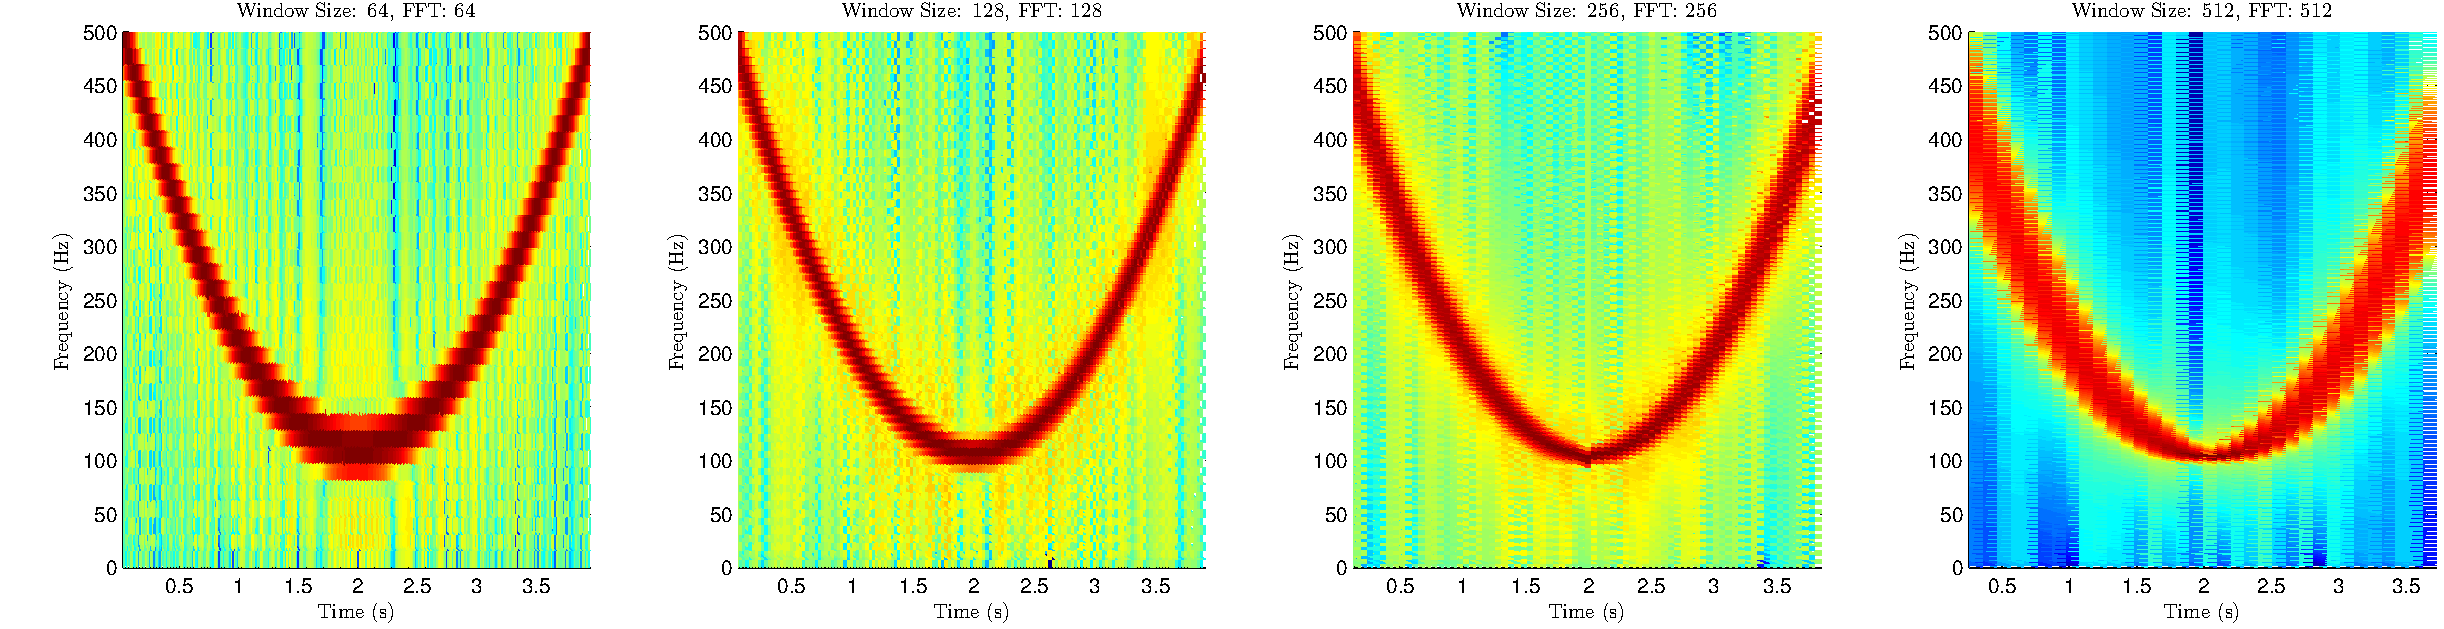
\includegraphics[scale=0.45]{fig/2/2_3_a_window_size.pdf}
	\caption{\textit{Differing Window Sizes}}
	\label{fig:2_3_a_window_size}
\end{figure}

\begin{figure}[h]
	\centering 
	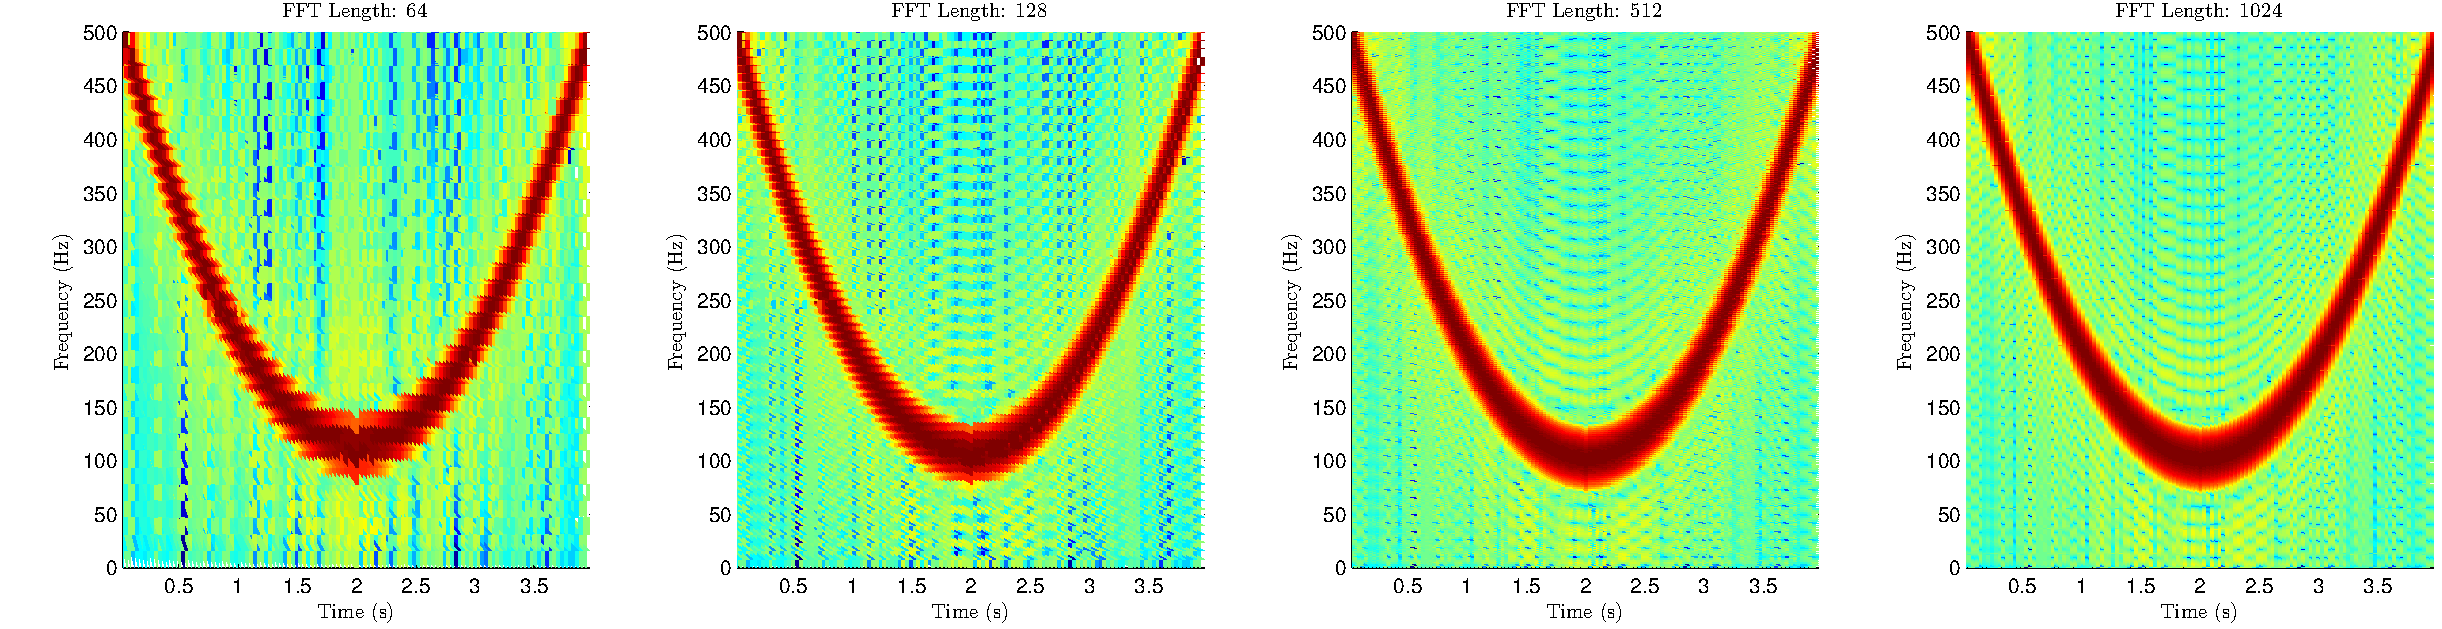
\includegraphics[scale=0.45]{fig/2/2_3_a_fft_len.pdf}
	\caption{\textit{Differing FFT lengths}}
	\label{fig:2_3_a_fft_len}
\end{figure}

\begin{figure}[h]
	\centering 
	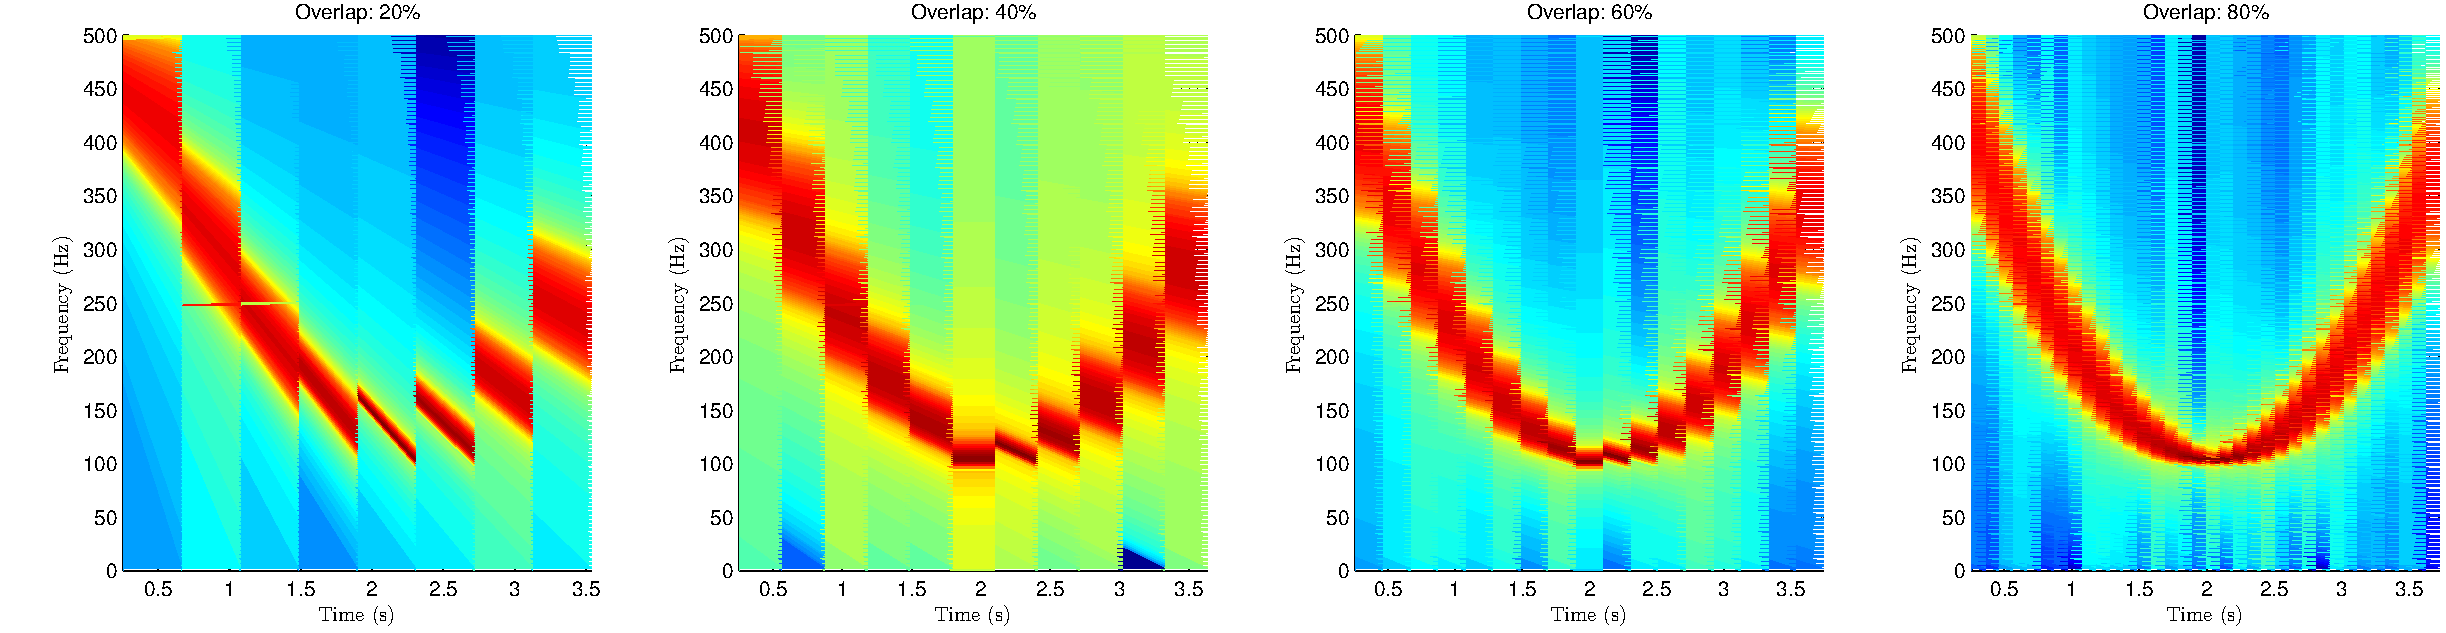
\includegraphics[scale=0.45]{fig/2/2_3_a_overlap.pdf}
	\caption{\textit{Differing Window overlaps}}
	\label{fig:2_3_a_overlap}
\end{figure}

\begin{figure}[h]
	\centering 
	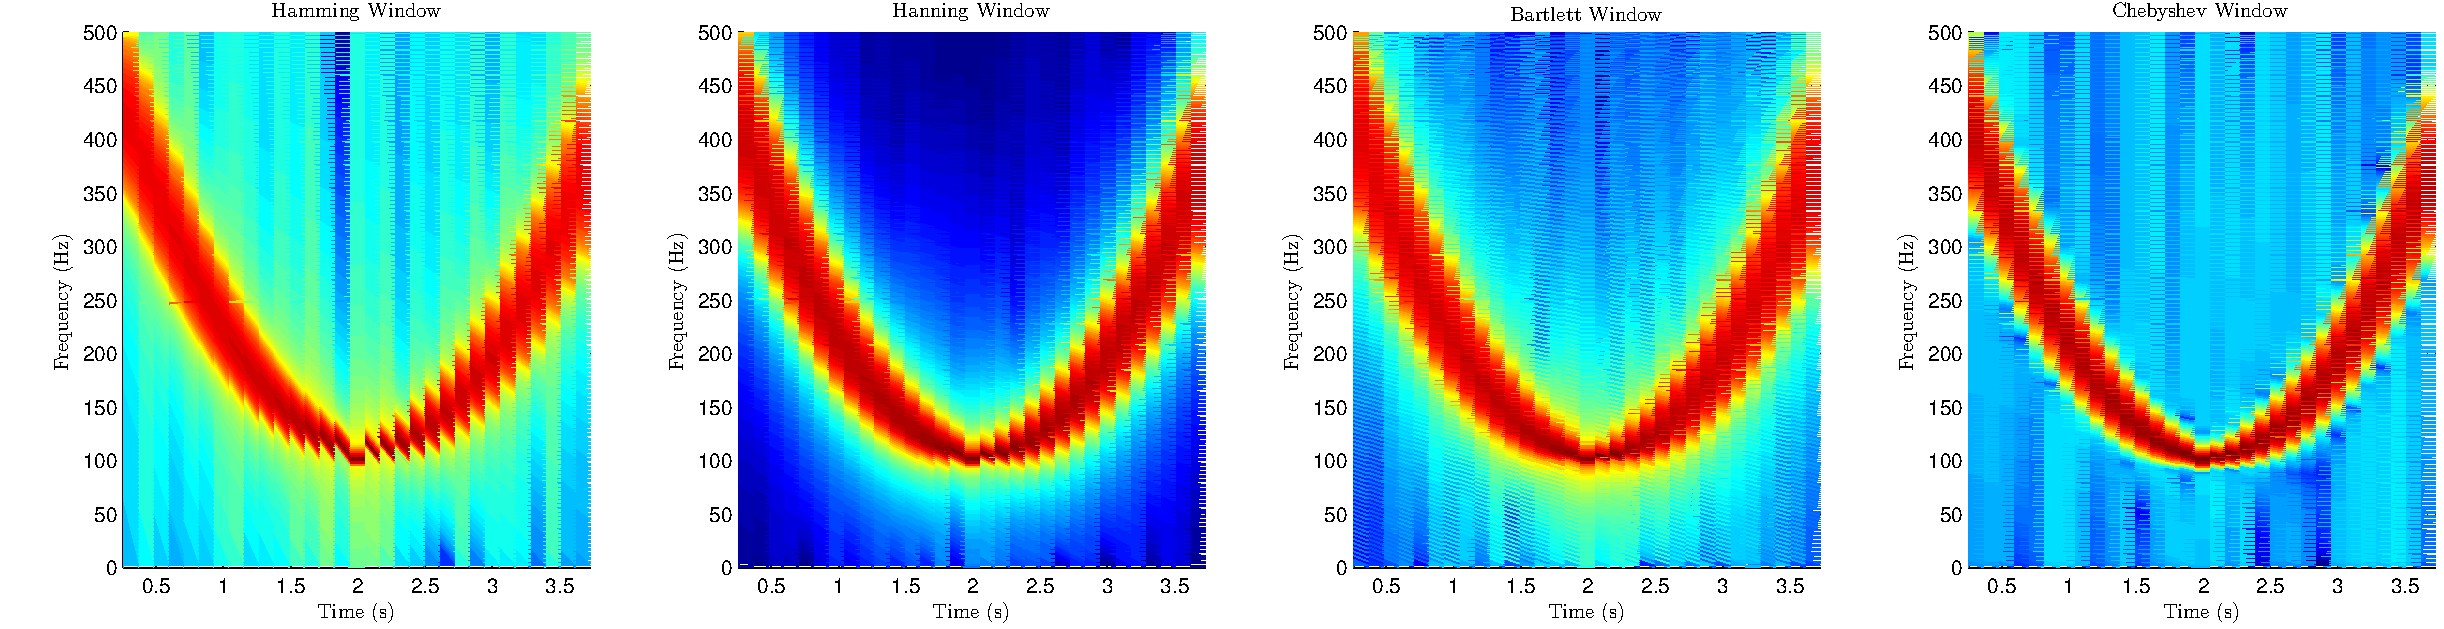
\includegraphics[scale=0.45]{fig/2/2_3_a_windows.pdf}
	\caption{\textit{Different window functions}}
	\label{fig:2_3_a_windows}
\end{figure}

\subsubsection{Spectrogram of Real-World EEG Data}

Having understood the basics of how to create a spectrogram, we now look at creating one for some real-world data. In this case, an EEG signal. In order to achieve good spectral resolution, which pick an FFT length of 4096, nearly four times the sampling frequency (1200$Hz$). Based on the performance in tests conducted, a window length of $\sim$ 75\% was selected (3000 samples). The Hanning window performed best in the last spectrogram test, so was also used here.

Figure \ref{fig:2_3_b} shows the final spectrogram. We appear to have good frequency and time performance. We can see very clearly the 50Hz mains interference, as well as activitiy between 10 and 20$Hz$. We also have the spectral resolution to observe the 13$Hz$ line, which otherwise may have been blurred in with the high amplitude noise nearer 10$Hz$.

\begin{figure}[h]
	\centering 
	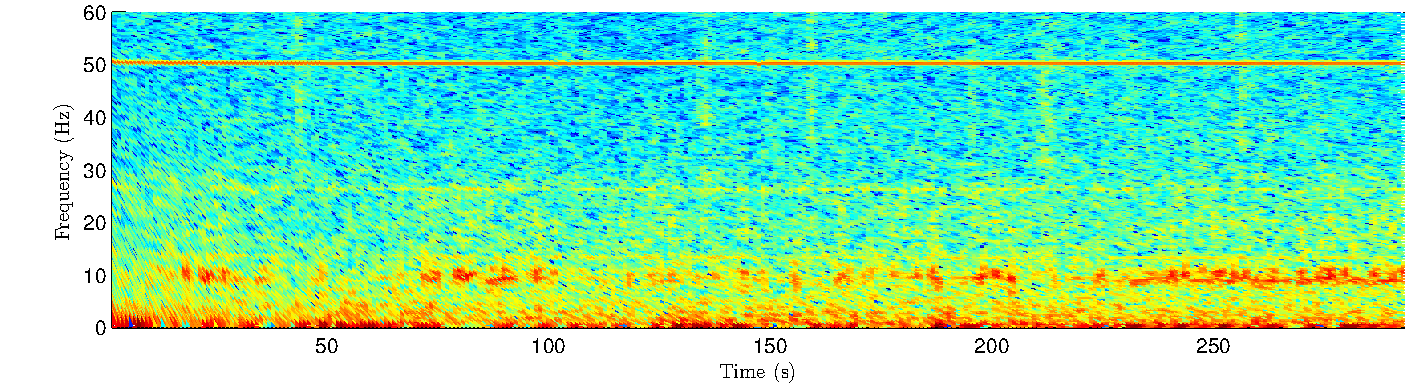
\includegraphics[scale=0.8]{fig/2/2_3_b.pdf}
	\caption{\textit{Spectrogram of EEG data}}
	\label{fig:2_3_b}
\end{figure}

\end{document}

